\chapter{Energy-Based Models}
% Authors: Bofeng Hu (Editor), Sakada Lim, Jialing Liao
% Lecture  points e: 3/25/2019

\section{Introduction}
% Authors: Bofeng Hu (Editor), Sakada Lim, Jialing Liao
% Lecture date: 3/25/2019

The Energy-Based Models (EBM) approach provides a general framework for many machine learning algorithms. 
They are designed to deal with situations where the machine learning system does not just compute an output as in a feed-forward process, but computes an output as the result of some optimization.

There are two forms of EBM, one for supervised learning (conditional) and one for unsupervised learning (unconditional). 
The conditional models take $X$ and $Y$ as input, while the unconditional models take only $Y$ as input. 
Their outputs are scalars, $F(X,Y)$ or $F(Y)$.


\begin{figure}[htb]
    \centering
    \begin{subfigure}[b]{0.25\textwidth}
        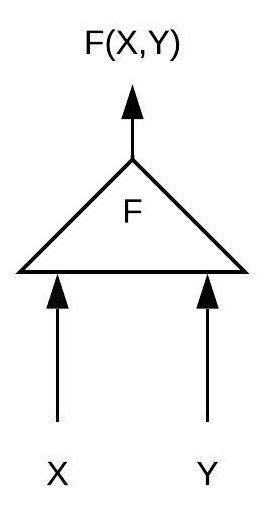
\includegraphics[width=\textwidth]{figs/EBM1-2.jpeg}
        \caption{Conditional}
        \label{fig:conditional}
    \end{subfigure}
    \begin{subfigure}[b]{0.27\textwidth}
        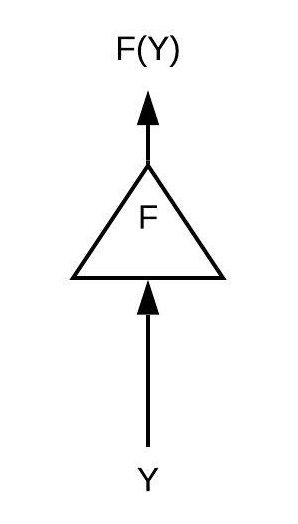
\includegraphics[width=\textwidth]{figs/EBM2-2.jpeg}
        \caption{Unconditional}
        \label{fig:unconditional}
    \end{subfigure}
    \caption{Two forms of Energy-Based Models}\label{fig:EBM}
\end{figure}

The output value indicates the ``compatibility'' of the input. 
In the conditional case, assume we have a properly trained EBM, and we show it an image of a table and the label for table, we get a small value as output, indicating these two are compatible. 
If we use an image of a table and the label for car, then the output energy should be higher. 
In the unconditional case, there is only one input, and the model tells us if it "looks good". 
For example, if this model is trained on natural images (ImageNet), and we show it an image like those in ImageNet, we get a low energy. 
But if we show it noise or something not natural, we get a high energy.


The model can be viewed as an energy function $F$. 
Suppose $X$ and $Y$ are both scalars, and the data points are two-dimensional like in ~\cref{fig:conditionalexample1} and ~\cref{fig:unconditionalexample1}. 
In the conditional case, We want a function that takes low values on observed points and high values elsewhere. 
The problem is that for the value of $X$ at the bar, there are two possible $Y$. 
If we build a model, for example a neural network, and compute $Y$, we can only get one value for $Y$. 
How do we represent the fact that we have two $Y$? One trick is that we go through an implicit function. 
When we want to parameterized a circle, we use $X^2+Y^2=r^2$. 
We can design an energy function that looks like $(X^2+Y^2-r^2)^2$, which takes value 0 on the circle and larger values inside or outside the circle. 
This is one problem EBM attempts to solve. 
In the unconditional case, instead of $X$ and $Y$, we have two $Y$. 
Instead of predicting $Y$ from $X$, we might have to predict $Y_1$ from $Y_2$ or $Y_2$ from $Y_1$ or just how they are compatible with each other. 

\begin{figure}[htb]
    \centering
    \begin{subfigure}[b]{0.3\textwidth}
        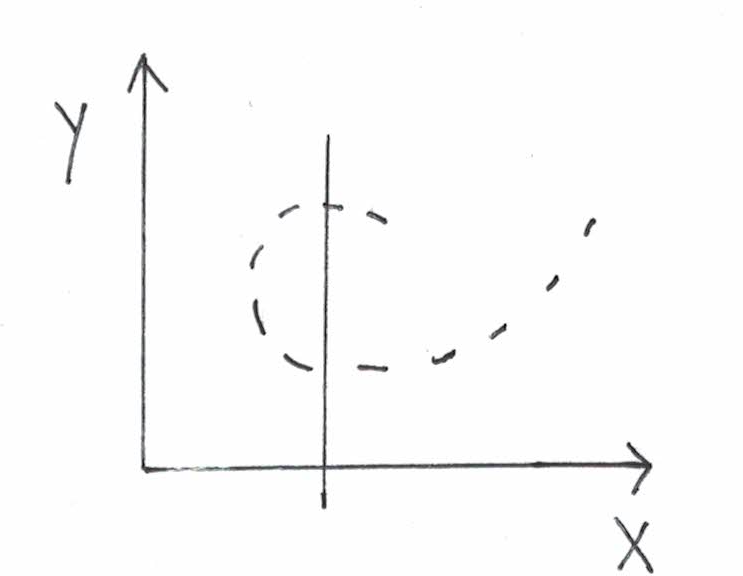
\includegraphics[width=\textwidth]{figs/EBM3.png}
        \caption{Conditional}
        \label{fig:conditionalexample1}
    \end{subfigure}
    \begin{subfigure}[b]{0.29\textwidth}
        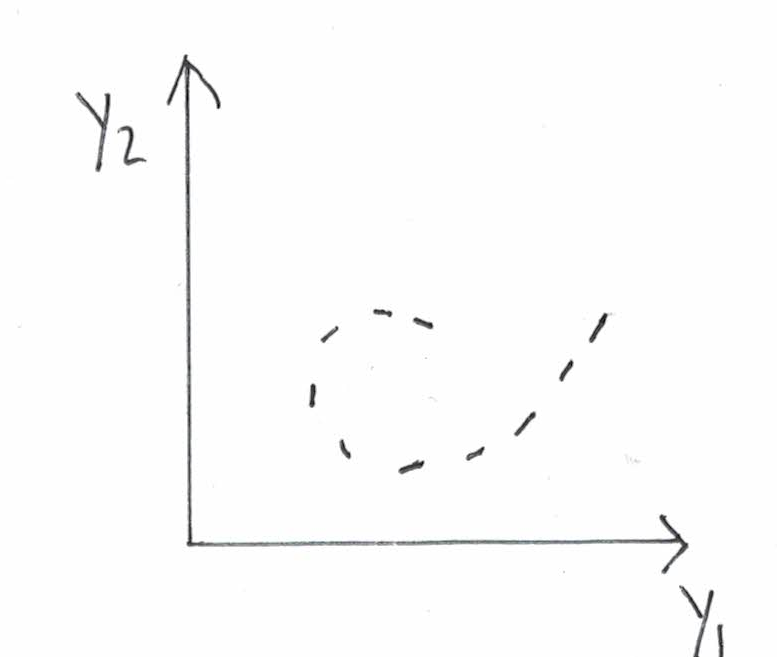
\includegraphics[width=\textwidth]{figs/EBM4.png}
        \caption{Unconditional}
        \label{fig:unconditionalexample1}
    \end{subfigure}
    \caption{Usage of EBM}\label{fig:Example1}
\end{figure}


For the above problems, we want some energy function that looks like \cref{fig:energyfunction}. 
The darker area represents the valley. When we move away from the valley, our energy goes up. 
For predicting $Y$ from $X$, We can just find where our $Y$ has the lowest energy.

\begin{figure}[htb]
  \centering
    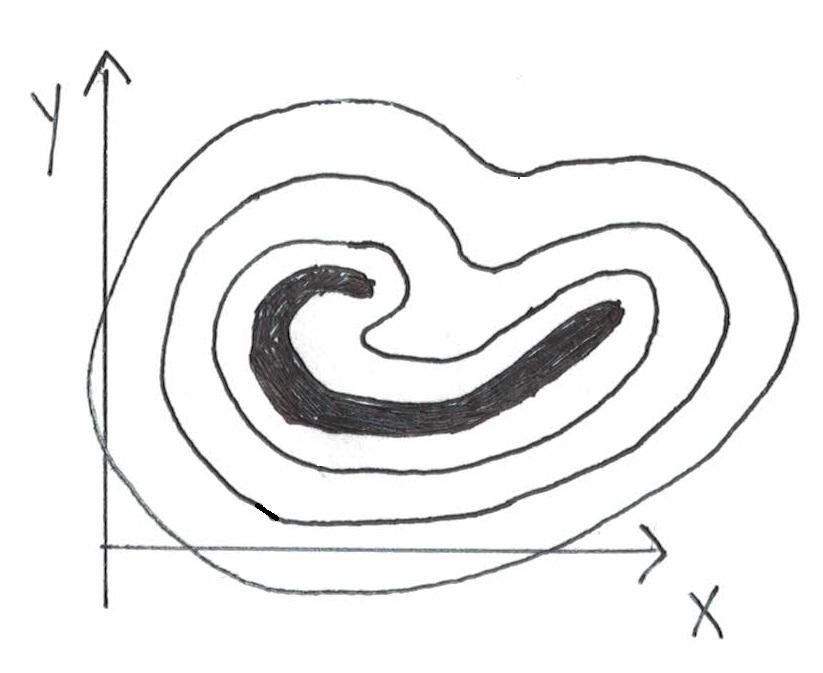
\includegraphics[width=0.3\textwidth]{figs/EBM5.png}
    \caption{Energy Function}
    \label{fig:energyfunction}
\end{figure}

\subsection{Relation with Probabilistic Models}
% Authors: Bofeng Hu (Editor), Sakada Lim, Jialing Liao
% Lecture date: 3/25/2019
If we want to turn an EBM into a probabilistic model, like $P(Y|X)$. We can parameterized it with:


\begin{equation*}
    P(Y|X) = \frac{e^{-\beta F(X,Y)}}{\int_y e^{-\beta F(y,X)}}
\end{equation*}

Now we are turning an energy which we have not specified positive or negative into positive. 
Here the integral is over the entire space of $Y$, so this is a normalized distribution over $Y$. 
This is called the (Gibbs) Boltzmann distribution, which comes from statistical physics. 
This is a way of transforming an energy function into a distribution. 
But the normalization term is not always tractable. 
$y$ might be in high-dimension space. 
The energy function does not have a easy-to-compute integral, and so the normalization term is not computable. We have to use tricks like variational methods or Markov chain Monte Carlo. But this would make it complicated.

\subsection{Energy-Based Inference}
% Authors: Bofeng Hu (Editor), Sakada Lim, Jialing Liao
% Lecture date: 3/25/2019
In the conditional case, the inference process is to find a $Y$ which minimizes this $F$ function. like

\begin{equation*}
    Y^* = \argmin_y F_w (X,Y)
\end{equation*}

Note that there can be multiple minima.
When designing the $F$ function, its range can be lower bounded, like the square function, so we know 0 is the floor, and can make it larger for other things. 

Another kind of inference would be returning a distribution over $Y$ instead of a single $Y$. But the machine has to be trained a particular way.

The $F$ function is not minimized during training, but instead during inference. 
For training, we shall minimize another loss function. We are going to parameterized $F$ with w and train it.


\begin{figure}[htb]
    \centering
    \begin{subfigure}[b]{0.2\textwidth}
        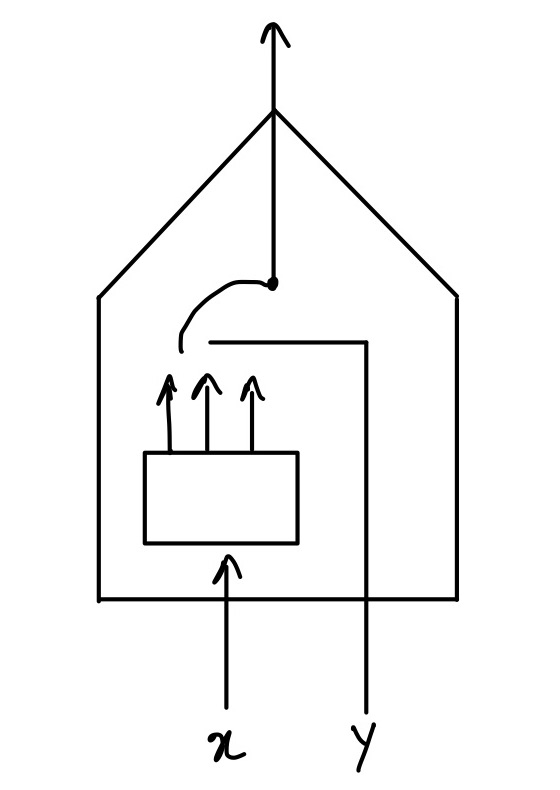
\includegraphics[width=\textwidth]{figs/EBM6-2.jpg}
        \caption{Conditional}
        \label{fig:energybasedmodel1}
    \end{subfigure}
    \begin{subfigure}[b]{0.2\textwidth}
        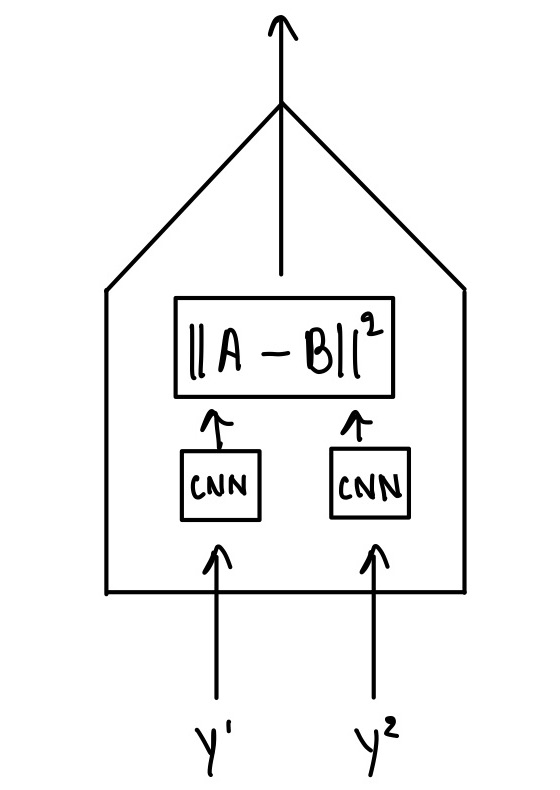
\includegraphics[width=\textwidth]{figs/EBM7-2.jpg}
        \caption{Unconditional}
        \label{fig:energybasedmodel2}
    \end{subfigure}
    \caption{Two examples of Energy-Based Models}\label{fig:Example2}
\end{figure}

In \cref{fig:energybasedmodel1}, the EBM takes an image, and run through a CNN which produces a bunch of scores for some categories. 
The $Y$ is a discrete variable, which acts like a switch and chooses which output of the CNN is propagated to the final output. 
Suppose we have three categories: table, car, airplane. 
When we show it an image of car, and put car in $Y$, it will select the output of car from the CNN, and return a score. A high score is bad, and a small score is good. 
If we put the label table, car and airplane in $Y$, we select each of those, and get their scores. 
If we want to know which one it is, we find the one which gives the lowest energy, and this will be the answer.

In \cref{fig:energybasedmodel2}, we feed two vectors $\vect{Y^1}$ and $\vect{Y^2}$, and ask the system if they are compatible. 
We run them both through CNN, and compute the distance between the two outputs. 
This can be used in a face detector, where the model gives low energy for faces of the same person and high energy for faces of different person.

\section{Energy-Based Training}
% Authors: Bofeng Hu (Editor), Sakada Lim, Jialing Liao
% Lecture date: 3/25/2019
The training process should return a function like this: When we have training samples like $(x^i,y^i)$, we want $F(x^i,y^i)$ to be small. 
At the same time, we want $F(x^i,y^j)$ to be large, where $i \neq j$. 
For the unconditional case, we want $F(y^i)$ to be small.

\begin{equation*}
Conditional \begin{cases}
    F_w(x^i,y^i), & \text{small}.\\
    F_w(x^i,y^j), & \text{$i\neq j$,larger}.
    \end{cases}
\end{equation*}

\begin{equation*}
Unconditional \begin{cases}
    F_w(y^i), & \text{small}.\\
    F_w(y)& \text{$y\neq y^i$, larger}.\\
  \end{cases}
\end{equation*}

We need an objective function which push down the energy of training samples, and another term that pushes up the energy of everything else (outside the training samples). 

Suppose we want an energy function that looks like \cref{fig:energyfunction}. 
The training samples will be in the valley region. After getting a training sample, we can tweak the parameters of the energy function by gradient descent, so that the output energy goes down.

How do we push up the energy outside? 
We can generate samples outside and push them up. 
The space outside can be large, but this is what probabilistic approaches do.

Say we believe in maximum likelihood. 
Suppose we parameterized $P(Y|X)$ with a Boltzmann distribution.

\begin{equation*}
    P_w(Y|X) = \frac{e^{-\beta F_w(X,Y)}}{\int_y e^{-\beta_w F(y,X)}}
\end{equation*}

We want to maximize the probability over the training samples

\begin{equation*}
    \prod_{i} P(y^i|x^i)
\end{equation*}

That is, we want to minimize the negative log of it.

\begin{equation*}
    L(w) = -\sum_i \log P(y^i | x^i)
\end{equation*}

That is our objective function. We plug in the distribution and rename this function, we get

\begin{equation*}
    \begin{split}
        L(w) & = \sum_i -\log \bigg\lbrack\frac{e^{-\beta F_w(x^i,y^i)}}{\int_y e^{-\beta_w F(y,x^i)}}\bigg\rbrack \\
        & = \sum_i [-\log e^{-\beta F(x^i,y^i)} + \log\int_y e^{-\beta F_w(x^i,y^i)}]
    \end{split}
\end{equation*}

\begin{equation*}
    \begin{split}
        L^{'}(w) & = \frac{1}{\beta}L(w) \\
        & = \sum_i [F_w (x^i,y^i) + \frac{1}{\beta}\log\int_y e^{-\beta F_w(y,x^i)}]
    \end{split}
\end{equation*}

When we try to minimize this, the first term tries to make the energy of the correct $y$ small, while the second term will make the energy of all $y$ high. 

If we compute the gradient with respect to $w$

\begin{equation*}
    \frac{\partial L(w)}{\partial w} = \sum_{i} [\frac{\partial F_{w}(x^i,y^i)}{\partial w} - \int_y P_{w}(y|x^i)\frac{\partial F_w(x^i,y)}{\partial w}]
\end{equation*}

where $P_w(y|x^i)$ is obtained through the Gibbs distribution.

There is a negative sign before the second term, which means it will increase the energy of all the y to some extent. 
More generally, what the gradient indicates is that, we are pushing down on the energy of the correct answer in the first term, and pushing up the energy of every answer, including the correct one, in the second term. 
And the force we push up a particular $y$ is proportional to the probability our model gives to that $y$. Note that the first term pushes down the energy of correct answers with a larger force.

If you have the energy function and can calculate the normalized term, then this is the way for maximizing the likelihood of the data, using the negative log-likelihood function.

If we take the EBM for \cref{fig:energybasedmodel1}, and we assume the probability of one $y$ given by the model is according to the Gibbs distribution. 
Suppose we try to push down the energy of the correct answers and push up the energy of the incorrect answers. 
Then this objective function becomes negative log-softmax, and this model is equivalent to a softmax on top of a neural network. 
We can also use other loss functions with similar results.

As it is difficult to parameterize $F$, we may use Monte Carlo methods to approximate the integral, for example using $\sum_{k} \frac{\partial F_w(x_i,y^k)}{\partial w}$. Another form of Monte Carlo is called Markov chain Monte Carlo (MCMC), where we have a sample $y$, and we modify the sample each time in such a way that every modification gives a sample that is more likely under the distribution. Another category for approximation is called variational methods, where we assume $P$ to have simpler form (e.g. Gaussian).

Basically, any object function that pushes down the energy of correct answers and pushes up the energy of incorrect answers will work. It may not be related to probabilities.

Fomally, energy based models can be summarize with the following procedure
\begin{enumerate}
    \item Design an architecture: Decide the form of E(W, Y, X)
    \item Pick an inference algorithm: Decide the method to find Y that minimize E(W, Y, X)
    \item Pick a loss function: Decide the function that measures E(W, Y, X)
    \item Pick an optimization method: Decide The method for finding W that minimizes $\mathcal{L}$
\end{enumerate} 

An important problem is how to decide the loss function for energy based models, and we will introduce different kind of loss functions in the following section.

\section{Energy Loss}
% Authors: Chiao-Hsun Wang
% Lecture date: 4/01/2019


A simple example for loss function is the energy loss. For a given training sample
$(X^i,Y^i)$, the loss is defined as
\[
    \mathcal{L}_{energy}(Y^i, E(W, \mathcal{Y}, X^i)) = E(W, Y^i, X^i)    
\]
Minimize the loss function corresponds to pulling down the energy of 
the correct answer. The problem is that training with the loss function won't
necessarily pull up the energy with respect to incorrect answers, which 
leads to a collapsed solution in some cases, 
where the model learns to set the energy as zero. 

\subsection{Negative Log-likelihood Loss}

The negative log-likelihood loss is defined as
\[
    \mathcal{L}_{nll}(W \mathcal{s}) = \frac{1}{P} \sum_i^P (E(W, Y^i, X^i) 
    + \frac{1}{\beta} \log \int_{y \in \mathcal{Y}} e^{-\beta E(W, y, X^i)}
\]

The idea is to maximize the conditional probabilities of all the
correct outputs Y given the input X in the training set, 
\[
    P(Y^1, Y^2, ..., Y^p |X^1, ..., X^p, W)
\]
Assuming the samples are independent and use Gibbs distribution
to transform energy into probabilities,
\[
    P(Y|X^i, W) = \frac{e^{-\beta E(W, Y, X^i)}}
    {\int_{y \in \mathcal{Y}}e^{-\beta E(W, y, X^i)}}    
\]
we will result in the equation
for negative log-likelihood loss.\\

The gradient of the negative log-likelihood loss for a single sample is 
\[
    \frac{\partial{\mathcal{L}(W, Y^i, X^i)}}{\partial{W}}
    = \frac{\partial{E(W, Y^i, X^i)}}{\partial{W}}
    - \int_{Y \in \mathcal{Y}} \frac{\partial{E(W, Y^i, X^i)}}{\partial{W}} P(Y|X^i, W)
\]
where $P(Y|X^i, W)$ is the Gibbs distribution.\\

\subsection{Perceptron Loss}

The perceptron loss is defined as 
\[
    \mathcal{\mathcal{L}}_{\text{perceptron}}(Y^i, E(W,\mathcal{Y}, X^i))
    = E(W, Y^i, X^i) - \min_{y \in \mathcal{Y}} E(W, Y, X^i)
\]

The intuition is from the perceptron algorithm,
which can be viewed as an energy based model.
\begin{itemize}
    \item Energy: $E(W, Y, X) = -YG_W(X)$
    \item Inference: $Y^* = sign(G_W(X))$
    \item Loss: $\mathcal{\mathcal{L}}_{\text{perceptron}}(W, \mathcal{S})
     = \frac{1}{P} \sum_{i=1}^P(sign(G_W(X^i))-Y^i)G_W(X^i)$
    \item Learning Rule: $W \leftarrow W + \eta (Y^i -sign(G_W(X^i)))
    \frac{\partial{G_W(X^i)}}{\partial{W}}$
\end{itemize}

The problem for perceptron loss is similar to energy loss,
where it may produce flat energy surface for certain cases.

\subsection{Generalized Margin Loss}

There are several loss functions that are described as general margin loss.
To introduce the concept, we need to first gives the definition 
to the "Most offending Incorrect Answer"\\

\textbf{Definition: } Let Y be a discrete variable. Then for a training sample $(X^i, Y^i)$,
the most offending incorrect answer $\bar{Y}^i$
is the answer that has the lowest energy among all answers that are incorrect:
\[
    \bar{Y}^i = \text{argmin}_{y \in \mathcal{Y}, Y \neq Y^i}
    E(W, Y, X^i)
\]
\\
\textbf{Definition: } Let Y be a continuous variable. 
Then for a training sample $(X^i, Y^i)$,
the most offending incorrect answer $\bar{Y}^i$
is the answer that has the lowest energy among all answers
that are at least $\epsilon$ away from the correct answer:
\[
    \bar{Y}^i = \text{argmin}_{y \in \mathcal{Y}, \parallel	Y-Y^i\parallel > \epsilon}
    E(W, Y, X^i)
\]
\\
Now we give several examples for generalized marginal loss.
\begin{itemize}
    \item Hinge Loss: 
    $L_{hinge}(W, Y^i, X^i) = \max(0, m + E(W, Y^i, X^i) - E(W, \bar{Y}^i, X^i))$
    \item Log Loss:
    $L_{log}(W, Y^i, X^i) = \log(1 + e^{E(W, Y^i, X^i) - E(W, \bar{Y}^i, X^i)})$
    \item Square-Square Loss:
    $L_{sq-sq}(W, Y^i, X^i) = E(W, Y^i, X^i)^2 + (\max(0, m - E(W, \bar{Y}^i, X^i)))^2$

\end{itemize}

Here is a table \cref{fig:energy_based_models_loss_functions} that summarises some of the loss functions for energy based models.
\begin{figure}[h!]
    \centering
    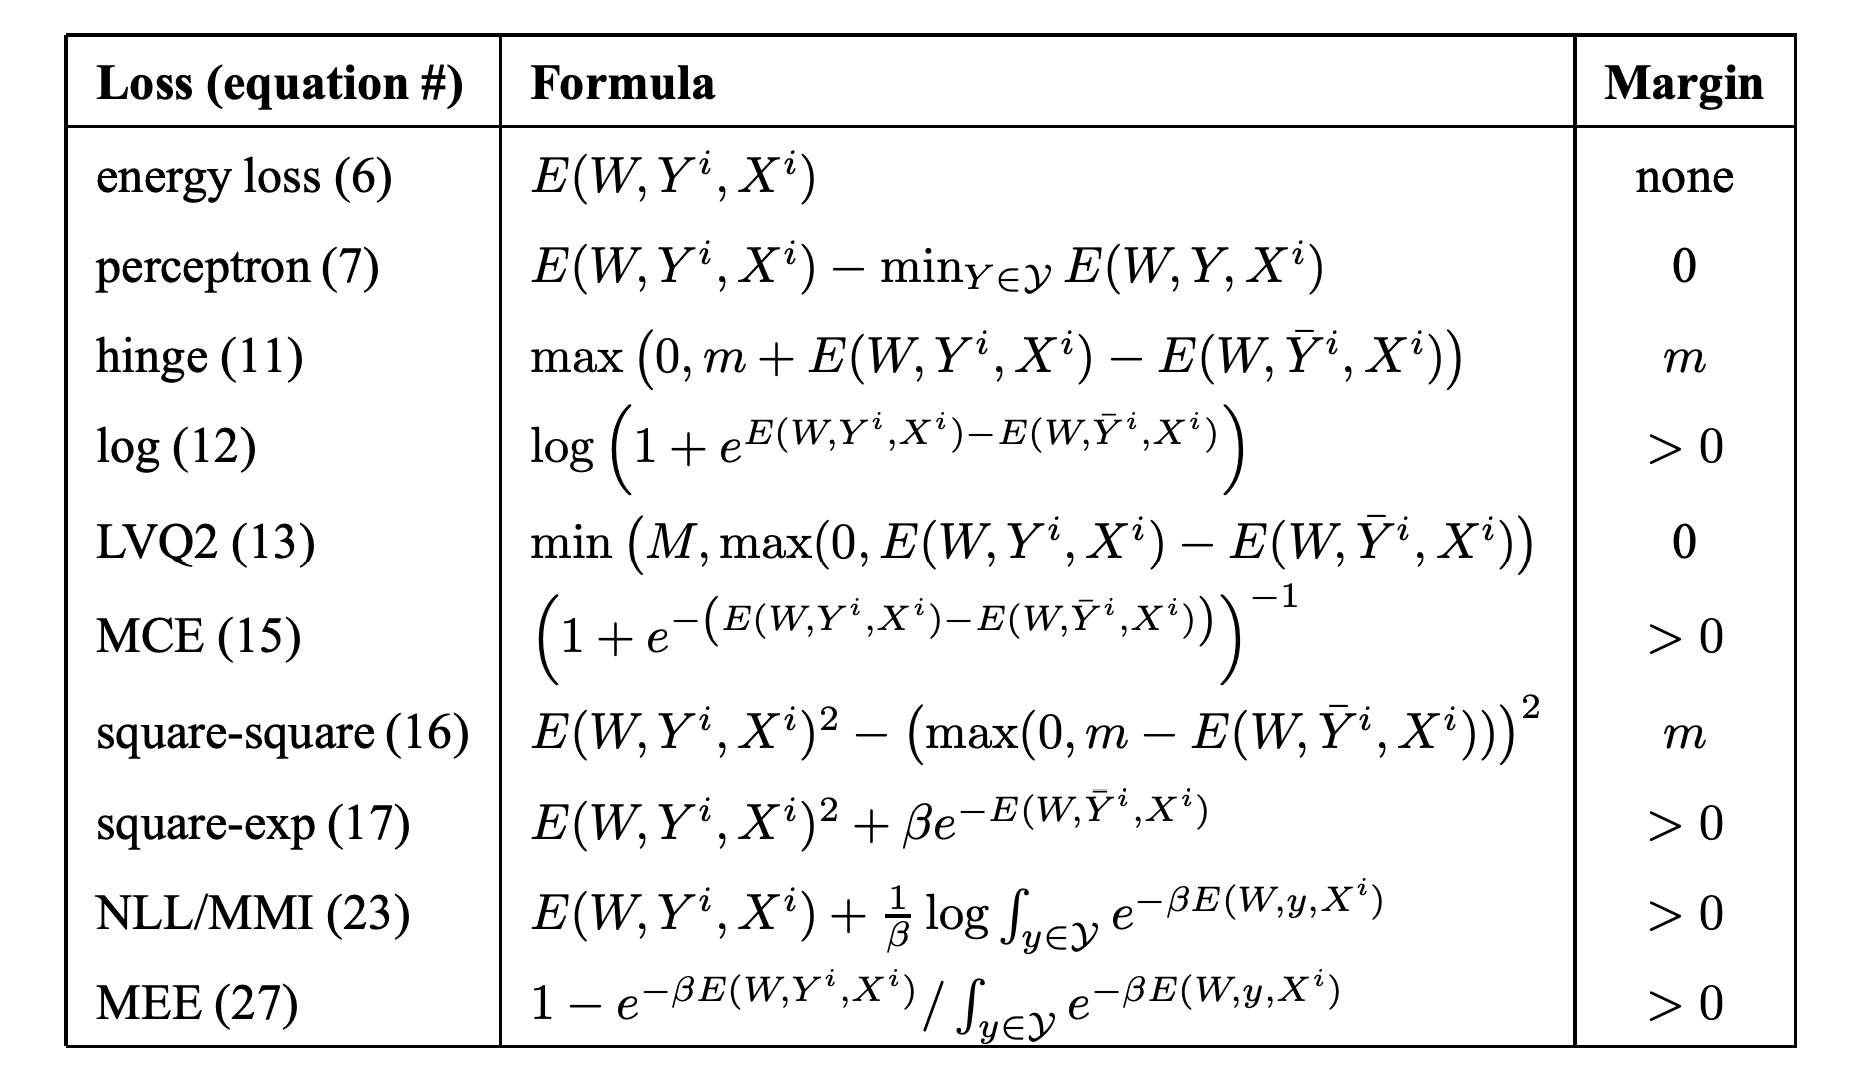
\includegraphics[width=300pt]{figs/loss_zoo.png}
    \caption{Different loss functions}
    \label{fig:energy_based_models_loss_functions}
\end{figure}









\newpage
\section{Latent Variable}
% Authors: Diksha Meghwal
% Lecture date: 04/01/2019
Often energy based models involve a third variable apart from the observed inputs which is not given but modelled into the architecture. These are called latent variables.
\begin{equation}
    F_{w}(Y) = min_{w} E(Y, Z)
\end{equation}
where $Z$ is not given.
\begin{figure}[!ht]
    \centering
    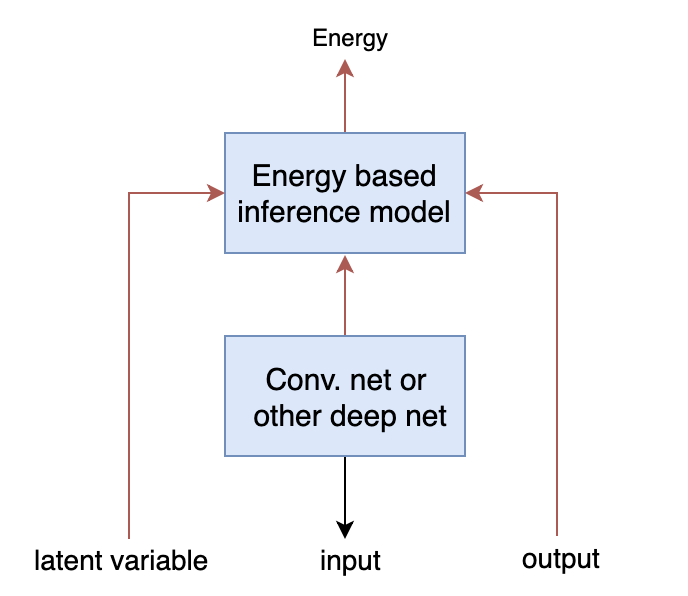
\includegraphics[width=0.4\linewidth]{figs/latent_EBM_architecture.png}
    \caption{latent EBM model}
    \label{fig:latent_EBM_model}
\end{figure}
\subsection{Examples}
\subsubsection{K-means clustering}
K-means clustering aims to partition n observations into k clusters in which each observation belongs to the cluster with the nearest mean, serving as a prototype of the cluster. This can be modelled as an energy based model where the energy function is given by:
\begin{equation}
    E_{w}(Y,Z) = \left\|Y - WZ \right \|^{2}
\end{equation}
where W is a matrix whose each column represents a prototype and Z is a one hot vector. So the value of this energy function gives the distance between the observed output and the prototype selected by the non-zero element in the vector $Z$.
And the inference for a sample is drawn using the function:
\begin{equation}
    F_{w}(Y) = \min_{Z \in one-hot-vector} E(Y, Z)
\end{equation}
Let 
\begin{equation}
    Z^{*} = \argmin_{Z} E_{w}(Y, Z)
\end{equation}
To calculate the loss function for all the samples we get the loss function:
\begin{equation}
    L(W) = \sum_{i}(F_{w}(Y^{i}))
\end{equation}
Derivating the loss function with respect to W we get:
\begin{equation}
    \frac{d}{dW} L(W) = \sum_{i}-(Y - WZ^{*}) Z^{*T}
\end{equation}
We use the above gradient to update the prototype matrix for each datapoint by considering the prototype that is closest to the datapoint and moving it a little closer to datapoint. Applying batch gradient descent on the above gradient to find the optimal solution gives us the K-means problem.

\subsubsection{Speech Recognition}
Speech recognition is also a classic exmaple of energy based models where the input is a sequence of data and the output is a sequence of feature vectors. We draw inference from these sequence of feature vectors using a language model. The top layer in this case is energy based models like Hidden Markov Chain or recurrent neural networks with some sampling mechanism.

\subsubsection{Keyword Recognition}
Keyword recognition involves detecting limited set of keywords from speech at a very fast rate. We model the problem that given a sequence of voice data, we try to determine the most likely word from the given small corpus. 
\begin{figure}[!ht]
    \centering
    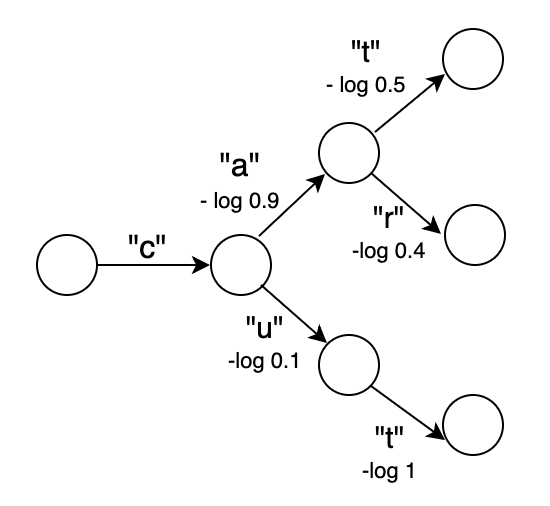
\includegraphics[width=0.4\linewidth]{figs/keyword model.png}
    \caption{keyword model with the cost for each choice marked on the edge}
    \label{fig:keyword_model}
\end{figure}
We use a small keyword dataset and assign cost to each next possible character in the dataset using a pre-trained language model as shown in the fig \cref{fig:keyword_model}. The cost of the word path is given by the combination of the cost of each step. We use a convolutional neural network or deep net to product cost for every possible sound at every time step and the model combine these energies with the energies provided by the pre-trained model and output the path with minimum cost. In this whole process of finding the solution, the latent variable is the cost of the path.

\subsubsection{Semantic Segmentation}
Semantic segmentation problems require that certain properties are maintained between the input and the output. We can force these restrictions using energy based models which give high energy to small areas of pixels that have a different category as compared to pixels of the large surrounding area. This ensures that there is some uniformity of categories in the output and the input.

\subsection{Marginalization}
As discussed earlier, for certain problems for whom the cumulative probability distribution converges,  we can use a probabilistic model based on Boltzmann distribution to draw the inference.
Considering the probability function:
\begin{equation}
    P(Y|X) = \dfrac{\exp^{-\beta F(X, Y)}}{\int_{y}\exp^{-\beta F(x,y)}}
\end{equation}
This equation can be re-written as:
\begin{equation}
    \int_{z}P(Y,Z|X) = \dfrac{\int_{z} \exp^{-\beta E(X,Y,Z)}}{\int_{y}\int_{z}\exp^{-\beta E(x,y,z)}}
\end{equation}
where Z is the latent variable. We now write this as:
\begin{equation}
    \int_{z}P(Y,Z|X) = \dfrac{\int_{z} \exp^{-\beta F(X,Y)}}{\int_{y}\exp^{-\beta F(x,y)}}
\end{equation}
where F is given by:
\begin{equation}
    F(X,Y) = -\dfrac{1}{\beta} \log \int_{z}\exp^{-\beta E(x,y,z)}
\end{equation}
Thus inference can be obtained by energy minimization over Y and Z given X.
The thing to note here is that the value of value of F(X,Y) is parameterised by $\beta$ and when $\lim_{\beta \to\infty} F_{\beta}(X,Y)$, the only terms that matter are those Y,Z in the power of $\exp$ which give the minimum value for energy,i.e.,:
\begin{equation}
    \lim_{\beta \to\infty} F_{\beta}(X,Y) = \min_{Z} E(X,Y,Z)
\end{equation}
As a result, in marginalization we end up combining all the values for all values of Z for a given Y that give the minimum energy as opposed to a simple probability based inference model where we just pick one value for a given X,Y.


